\documentclass{article}
\usepackage[utf8]{inputenc}
\usepackage{graphicx}
\usepackage{hyperref}
\graphicspath{{./images/}}

\title{LCBO Whisky Similarity Analysis}
\author{Nelson Siegel}
\date{August 2019}


\RequirePackage{filecontents}
\begin{filecontents}{mybib.bib}
@misc{word2vec,
    author= {{Chris Nicholson}},
    year  = {2019},
    title = {A Beginner's Guide to Word2Vec and Neural Word Embeddings},
    note  = {\url{https://skymind.ai/wiki/word2vec}, 
             Last accessed on 2019-08-24},
}
@misc{wordmover,
    author= {{Edward Ma}},
    year  = {2019},
    title = {Word Distance between Word Embeddings},
    note  = {\url{https://towardsdatascience.com/word-distance-between-word-embeddings-cc3e9cf1d632}, 
             Last accessed on 2019-08-24},
}

@misc{redditwhisky,
    author= {{Misc Reddit Users}},
    year  = {2019},
    title = {Reddit Whisky Network Review Archive},
    note  = {\url{https://docs.google.com/spreadsheets/d/1X1HTxkI6SqsdpNSkSSivMzpxNT-oeTbjFFDdEkXD30o}, 
             Last accessed on 2019-08-24},
}
\end{filecontents}

\bibliographystyle{plain}
\usepackage[hyphens,spaces]{url}

\begin{document}


\maketitle
\newpage
\tableofcontents
\newpage

\section{Introduction}

Finding good whiskies is difficult. Finding good whiskies for good prices is even more difficult! Finding good whiskies for good prices that are available at LCBO is almost impossible.

Thus the intent of this project was to develop a method for finding whiskies that are similar to ones that the user already prefers, but might be cheaper or better value.

In order to do this, data was collected from Reddit on whisky reviews, as well as data from LCBO. This data was combined, then a Word2Vec model was trained on the Reddit reviews. Next, similarity was calculated using Word Mover Distance with the trained Word2Vec model and generated for the entire dataset.

\section{Background}

Word2Vec is a shallow neural network that calculates similarities between two words by finding how often the occur near each other \cite{word2vec}. By training a Word2Vec model we can then run Word Mover Distance to calculate document similarity. 

Word Mover Distance matches up words in two documents in the method that creates the least "difference" between the documents \cite{wordmover}. See Figure \ref{fig:wordmoverdistance} for an example of how two completely different documents can have high similarity.

\begin{figure}[h]
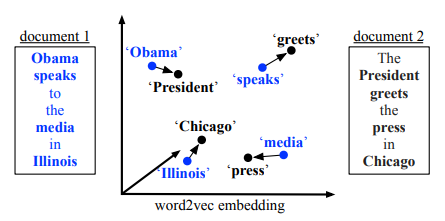
\includegraphics[width=\textwidth]{wordmoverdistance}
\centering
\caption{Word Mover distance matches similar words between documents \cite{wordmover}.}
\label{fig:wordmoverdistance}
\end{figure}

\newpage
\section{Research Question}
The intent of this analysis was to answer the following two questions:
\begin{enumerate}
    \item Given a whiskey that the user enjoys, how can we tell other whiskeys they will enjoy? The method used to determine is flavour similarity Word Mover Distance with Word2Vec on whisky review text.
    \item Based on the prices available for these whiskies at the LCBO, what is the best value purchase the user could choose that they would enjoy the most for the least cost? To do this a Rating per Price is displayed.
\end{enumerate}

\section{Methodology}

\subsection{Data Collection}

\subsubsection{Reddit Whisky Reviews}
In order to collect enough descriptive reviews to perform analysis, the Reddit Whisky Network Review Archive \cite{redditwhisky} was used to gain a list of Reddit reviews. Then full text was gathered using the praw wrapper for the Reddit api.

\subsubsection{LCBO Data}
To collect data for LCBO products was more difficult. There is no official documented LCBO api. Thankfully I was able to find an undocumented API at www.foodanddrink.ca, which is another LCBO run site. There are however, a few limitations to the API, most notably that you cannot search by product name but need to include a product number. As such I created a script that tried every possible product number and logged the results.

Another limitation is that a link to the LCBO site is not included from the API. In order to gather links from to the main LCBO api site, another script was required to search the LCBO site for the product number and grab the link.

\subsection{Modelling}

\subsubsection{Whisky Matchup}
One of the most difficult aspects of the project was combining the Reddit Whisky Review archive data with the LCBO data. This was difficult because whisky names are written differently. The general method that I ended up using was as follows:

\begin{itemize}
    \item Generate a list of keywords to search for. This was initially done by finding non-English words in whisky names but was later appended to include n-grams, as well as specific other words that could distinguish them, such as flavour types, special designations, or cask types.
    \item Each whisky in both Reddit and LCBO was then analysed to extract keywords as well as age from whiskies which had a defined match.
    \item All whiskies in the two datasets that had the exact same keywords as well as the exact same age were matched. In cases where more than one whisky matched, the python library Fuzzywuzzy was used to use a fuzzy matching algorithm to find the most similar name.
\end{itemize}

\subsubsection{Word2Vec Training}

The Word2Vec model was trained on the text of all of the reviews. For each word, a list of similar words can be output. Figure \ref{fig:word2vec} shows an example of the results from the model.

\begin{figure}[h]
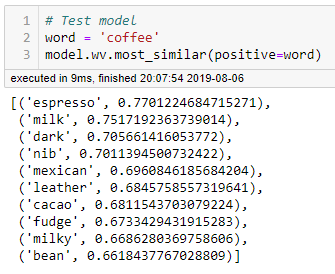
\includegraphics{word2vec}
\centering
\caption{Results from trained Word2Vec model for the word 'coffee'.}
\label{fig:word2vec}
\end{figure}  

\subsubsection{Word Reduction with TF-IDF}
In order to run Word Mover Distance in a reasonable amount of time, TF-IDF (Term Frequency, Inverse Document Frequency) was used to reduce the length of whisky descriptions. This was set to a limit of 50.

\subsubsection{Word Mover Distance}

Word Mover Distance was then run comparing every whisky to every other whisky. This was coded as a multicore process in order to decrease computation time as the number of whiskies exponentially increases the computation.

Figure \ref{fig:wordmover} shows the results for the Wild Turkey 101 Whisky.

\begin{figure}[h]
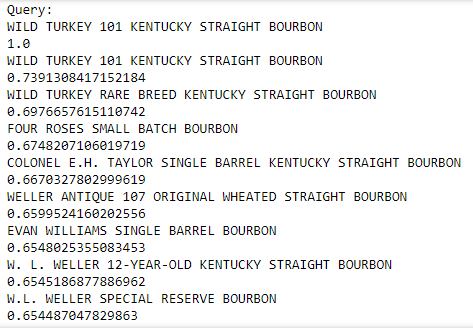
\includegraphics{wordmover}
\centering
\caption{Results from Word Mover Distance for the Wild Turkey 101.}
\label{fig:wordmover}
\end{figure}  

\subsection{App Development}
The app was developed as a Python Dash App. You can see an image of the App interface in Figure \ref{fig:app}

\begin{figure}[h]
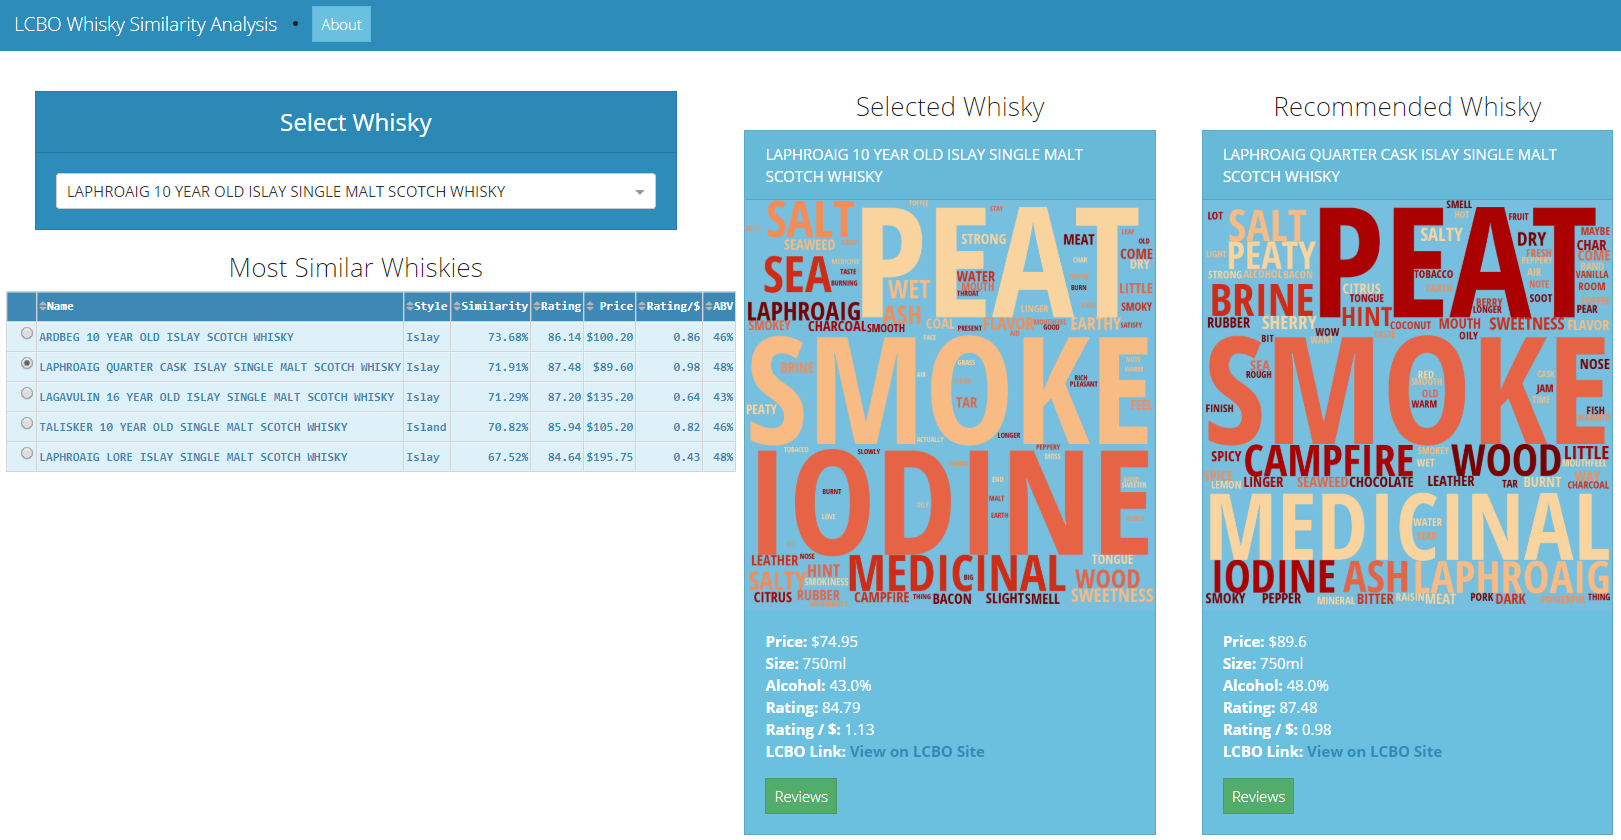
\includegraphics[width=\textwidth]{app}
\centering
\caption{App interface showing suggestions for Laphroaig 10.}
\label{fig:app}
\end{figure}  


\subsubsection{App Data}
To do this some of the data needed to be exported in the proper format. The following is a list of the datasets loaded by the app:

\begin{itemize}
    \item whisky\_tfidf.parquet : Basic whisky dataframe used to generate selector.
    \item whiskyinfo.parquet : Details about a whisky such as price, ABV, etc.
    \item similarities.parquet : Table showing every whisky's similarity to every other whisky.
    \item itemlinks.parquet : Table that includes an LCBO link for each whisky.
    \item reviewlist.parquet : Table that includes reddit review information and links for each whisky.
\end{itemize}

\subsubsection{App Function}

Within the App, there are several functions used to grab the required data to display to users. These are:

\begin{itemize}
    \item getReviews : Given an itemnumber, returns all reddit review information to populate a table.
    \item getLCBOLink : Given an itemnumber returns a link to the LCBO website.
    \item show\_top\_similarities : Returns table data of top n similar whiskies to selected itemnumber.
    \item getwhiskydesc : Given an itemnumber, returns all info to display to the user in a markdown format.
\end{itemize}

\newpage
\section{Results}

The results perform much better than I was expecting. Despite not guiding the algorithm at all by holding back regional styles, most suggestions fall within style boundaries, with exceptions being those whiskies that are outliers for their style, as would be expected. Figures \ref{fig:bourbon} and \ref{fig:irish} show examples of how Bourbons and Irish whiskies both recommend mostly the same category.

The app can be viewed at \href{https://lcbo-whisky-similarity.herokuapp.com/}{https://lcbo-whisky-similarity.herokuapp.com/}.

\begin{figure}[h]
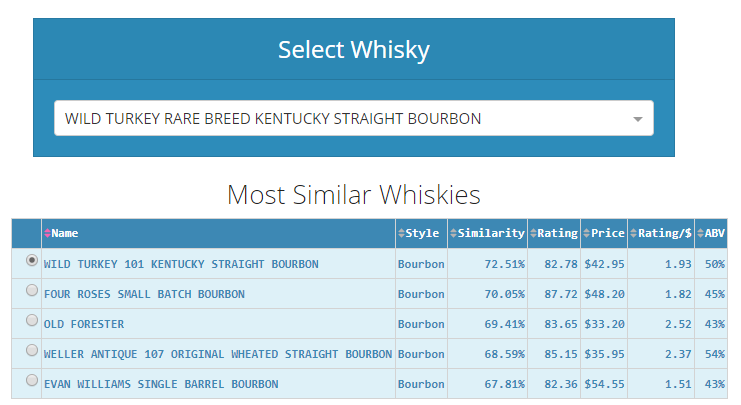
\includegraphics[width=\textwidth]{bourbon}
\centering
\caption{Suggestions for Wild Turkey Rare Breed.}
\label{fig:bourbon}
\end{figure}  

\begin{figure}[h]
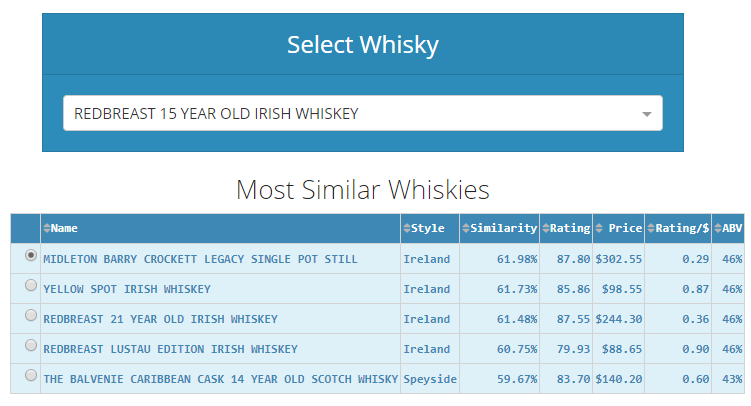
\includegraphics[width=\textwidth]{irish}
\centering
\caption{Suggestions for Redbreast 12.}
\label{fig:irish}
\end{figure}  

\newpage
\section{Discussion}
I am happy with the results and the recommendations given, as well as the app interface. Exploring the data through the app reveals a few issues with data cleaning that I would like to address, such as a couple of whiskies appearing twice, or some reviews being matched to other whiskies.

I would also like to improve on the process by implementing a database and having scripts run incrementally to capture new reviews and products.

\newpage
\bibliography{mybib}
\listoffigures
\end{document}
